\subsubsection{Q10.20 data 10312021 11092021 grouped by scenario \& Sex}

\begin{comment}
                      EFPR        EO      EFNR     n    pvalue
(frauth, Female)  0.531250  0.468750  0.500000  32.0  0.735498
(frauth, Male)    0.363636  0.636364  0.318182  11.0  0.405882
(icu, Female)     0.590909  0.409091  0.621212  33.0  0.165625
(icu, Male)       0.833333  0.166667  0.666667   3.0  0.157299
(rent, Female)    0.413793  0.586207  0.517241  29.0  0.298476
(rent, Male)      0.350000  0.650000  0.400000  10.0  0.267257
\end{comment}

\begin{table}[h]
    \centering
    \begin{tabular}{|c|c|c|c|c|c|c|}
        \hline
        scenario & Sex & EFPR & EO & EFNR & n & p-value\\
        \hline
        frauth & Female & \textbf{0.531} & 0.469 & 0.500 & 32.0 & 0.735\\
		frauth & Male & 0.364 & \textbf{0.636} & 0.318 & 11.0 & 0.406\\
		icu & Female & \textbf{0.591} & 0.409 & \textbf{0.621} & 33.0 & 0.166\\
		icu & Male & \textbf{0.833} & 0.167 & \textbf{0.667} & 3.0 & 0.157\\
		rent & Female & 0.414 & \textbf{0.586} & \textbf{0.517} & 29.0 & 0.298\\
		rent & Male & 0.350 & \textbf{0.650} & 0.400 & 10.0 & 0.267\\
		
        \hline
    \end{tabular}
    \caption{Grouped by scenario Sex}
    \label{tab:my_label}
\end{table}
\begin{figure}[h]
    \centering
    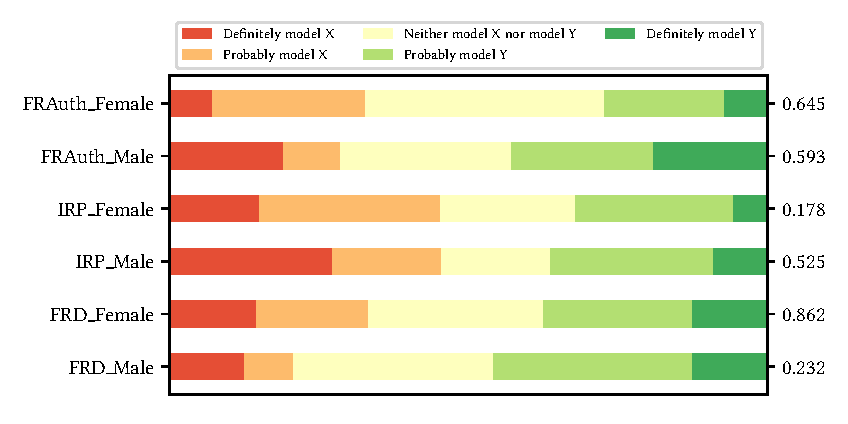
\includegraphics[width=0.8\textwidth]{figures/Q10.20/10312021_11092021/Q10.20_scenario_Sex.pdf}
    \caption{Grouped by scenario \& Sex}
    \label{fig:my_label}
\end{figure}
